\documentclass[12pt,a4paper]{ctexart}
\usepackage{enumitem}
\usepackage{float}
\usepackage{ulem} % 必须加载此宏包才能使用 \sout
\RequirePackage{graphicx}
\usepackage{fancyhdr}  % 导入页眉页脚配置宏包
\RequirePackage{hyperref}
% 关键:将默认英文前缀替换为中文前缀
\renewcommand{\figureautorefname}{图}    % 图片引用显示"图"
\renewcommand{\tableautorefname}{表}     % 表格引用显示"表"
\renewcommand{\equationautorefname}{式}  % 公式引用显示"式"
\renewcommand{\sectionautorefname}{节}   % 章节引用显示"节"
%\hypersetup{linktoc=all, colorlinks=true, linkcolor=black, urlcolor=black, citecolor=black, bookmarksnumbered, bookmarksopen=true}	% or

\hypersetup{linktoc=all, colorlinks=true, linkcolor=blue, urlcolor=blue, citecolor=blue, bookmarksnumbered, bookmarksopen=true}	% or

%%%%%%%%%%%%%%%%%%%%%%%%%%%%%%%%%%%

\begin{document}
% 标题页(单独一页)
\begin{titlepage}
  % 1. 顶部:插入学校Logo(需提前准备图片文件,如logo.png)

  \centering

        
\includegraphics[width=0.25\textwidth]{images/logo.png}  % 调整Logo宽度


      
    % 2. 中间:标题核心内容(居中)
    \vspace{2cm}  % 顶部到标题的间距
    \centering
    \Huge \bfseries 大连理工大学机械工程学院\\
    \vspace{0.5cm}
    \Huge \bfseries 博士毕业流程参考说明\\
    \vspace{4cm}  % 标题到作者的间距
    
    % 3. 底部:作者、日期(右对齐,更正式)

        \normalsize 作者:王小二的简单生活\\
        \vspace{0.3cm}
        
        修订日期:\today\\
        \vspace{0.3cm}
        
        版本:V1.1
        \vspace{0.3cm}
        
        最新文档地址。\href{https://github.com/DrHanks91/DUTMePhDProcess.git}{GitHub}

    
    % 底部留白
    \vfill
\end{titlepage}

% 正文从新页开始
\clearpage  % 可选,确保标题页完全结束后再开始正文

% 启用 fancy 样式
\pagestyle{fancy}

% 清空默认页眉页脚内容
\fancyhf{}

% 配置页眉内容(以居中显示文档标题为例)
\fancyhead[C]{大连理工大学机械工程学院-博士毕业流程参考说明}

% 配置页脚(居中显示页码)
\fancyfoot[C]{\thepage}
% 配置页脚(居中显示页码)
\fancyfoot[C]{\thepage}
% 添加页眉横线(关键配置)
\renewcommand{\headrulewidth}{1.5pt}  % 横线宽度(0pt 为隐藏)
\tableofcontents

\clearpage{}
\section*{写在前面}
\label{sec:pre}

此文档为仓促间完成,难免有疏漏和错误部分,仅作参考之用,若因本文档产生的意外、错误、甚至其他事故,本作者不承担任何责任,特此声明。

这个声明,你不同意, 下面就别看,也别参考,知道不。

本作者已经毕业,无法对文档进行持续更新。若有志同道和且愿意“接棒”继续更新文档者,可与作者联系,请发送邮件至\href{mailto:BusinessForQt@gmail.com}{BusinessForQt@gmail.com},并注明来意。

最新文档:\href{https://github.com/DrHanks91/DUTMePhDProcess}{大连理工大学机械工程学院-博士毕业流程参考说明}.

Pull Request:\href{https://github.com/DrHanks91/DUTMePhDProcess}{Pull Request}




\section{准备}
请自行查询是否满足答辩条件。有但不局限于:

\subsection{开题和中期}
\label{sec:kaiti}


参见\href{https://gs.dlut.edu.cn/info/1031/9635.htm}{大连理工大学研究生开题和中期考核管理规定}。

\subsection{博士生分流}
\label{sec:fenliu}

参见\href{https://gs.dlut.edu.cn/info/1079/8943.htm}{大连理工大学博士研究生分流管理办法(试行)}。

\subsection{结业考核}
\label{sec:jieye}

结业考核通过,即修完培养计划规定的课程学分,开题和中期考核通过。

自助打印成绩单。在研究生院、大学生活动中心、财务等各位置处均可打印。使用玉兰卡或身份证进行身份识别。此成绩单可以免费打印5份,后1.5元/份。建议打三份,一份上交(与学位申请书一起)、一份自留、一份备用。

硕博连读的学生须有硕博两阶段的成绩单。

样本如下:

\begin{figure}[H]
  \centering
  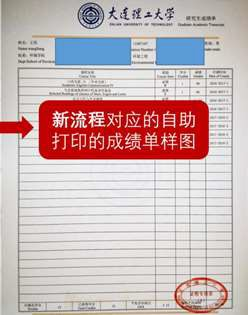
\includegraphics[width=0.3\textwidth]{images/meritList.jpg}  % 调整Logo宽度
  \caption{自助打印成绩单示例}
\end{figure}

\subsection{学制要求}
\label{sec:yearRequire}

\begin{enumerate}
\item 统考入学和申请考核制入学的学术学位博士研究生的基本学制为4 年,直博生的基本学制为5 年(含学习课程1 年),硕博连读博士生的基本学制为4 年(不含硕士2 年);
\item 各类全日制博士生在校修业年限为6 年,申请博士学位最长年限为8 年(含休学时间)
\item 研究生因参军入伍、创业休学的,其在校学习时间上限将根据审批时的约定和国家相关规定顺延。
\end{enumerate}


\subsection{发表论文要求}
\label{sec:paperRequire}

根据本学科专业,咨询韩愈老师。或根据以往毕业博士情况,一般来讲,自己课题组会加高一部分要求。

也可参见\href{https://gs.dlut.edu.cn/yjspy/xwgl12/fblwyq1.htm}{发表论文要求}。

\subsection{大论文准备}
\label{sec:thesisRequire}

根据自己研究方向和发表论文,撰写大论文。大论文一般为5章节,可参见博士论文模版\ref{sec:listRequire}小节。

论文可以使用方案排版软件Word或\LaTeX 撰写,模版可从研究生网站下载。Word优点是所见所得,不用麻烦配置任何东西,但后续改格式时,会像吃了屎一样,如公式、图表和排版等。\LaTeX 对公式、图表和排版相对友好,但前期投入精力多,前期像吃了屎样。所以,自己决定是前期吃屎还是后期吃屎。我是选择了前期吃。

\textbf{对于Word编写建议}:
\begin{itemize}
\item 软件:Office-Word
\item 文献管理软件:EndNote(推荐)、NoteExpress、Zotero、Mendeley等。
\item 引用格式:Endnote-\href{https://endnote.com/downloads/styles/chinese-standard-gb-t7714-numeric/?srsltid=AfmBOor20AgTDOjwFDm6fJqbAP8A6gGHeKBfwV-UuxWS9wOtau8e8W6M}{Chinese Standard GBT7714 (numeric)},需要稍微修改。请自行查找。
 \end{itemize}

  \textbf{对于\LaTeX 编写建议}:请先看自己导师是否同意,这个很重要。导师不看PDF和\LaTeX 文档,一切白瞎。真的,真会白瞎,你相信我。
  \begin{itemize}
    \item 编译器包:TexLive2024。
\item 软件:TexStudio。
\item 文献管理软件:Jabref。
\item 编译方式XeLaTeX ---  biber ---  XeLaTeX --- XeLaTeX 。
 \end{itemize}

 
 此外,可以使用我撰写的\LaTeX 模版。下载地址:大连理工大学博士论文\LaTeX 模版。下载地址:\href{https://github.com/DrHanks91/DUT_PhD_Thesis_Template}{大连理工大学机械工程学院博士论文LaTeX模版}。
 

 \subsection{表格与模版}
 \label{sec:listRequire}

一般会遇到以下文档:
 \begin{enumerate}
   \item \href{https://gs.dlut.edu.cn/info/1207/3994.htm}{大连理工大学博士学位申请流程}
 \item \href{https://gs.dlut.edu.cn/info/1210/13916.htm}{大连理工大学学位论文模版+格式规范}
\item \href{https://github.com/DrHanks91/DUTMePhDProcess}{答辩邀请卡片.docx-非必需}   
 \item \href{https://github.com/DrHanks91/DUTMePhDProcess}{机械工程学院博士学位论文内审审批表-韩愈版本}
 \item \href{https://gs.dlut.edu.cn/info/1207/8541.htm}{大连理工大学博士学位申请书(202504).doc}
 \item \href{https://gs.dlut.edu.cn/info/1207/8541.htm}{外审为B-C-D-E时修改说明评审意见表(202504).doc}
 \item \href{https://gs.dlut.edu.cn/info/1207/8541.htm}{大连理工大学博士学位论文答辩情况表 (202504).doc}
 \item \href{https://gs.dlut.edu.cn/info/1209/13422.htm}{各学部学院学位评定分委员会名单(202312-)}
 \end{enumerate}

 \subsection{补充}
\label{sec:auc}




所需要的文件在正文中需要的地方列出。
需要注意的有:
\begin{itemize}
\item 答辩系列表格里面的字体至少至5种\footnote{哕。},请注意自己本地电脑上是否安装。若不确定,宋体为保险字体。
\end{itemize}

\section{阶段1:内审/初审}
\label{sec:rev1}
完成论文初稿,且内审表导师签字。按照表格要求,发送到韩愈老师指定邮箱。以防万一,请发送后找韩愈老师核实是否收到。

韩愈老师会发送给本院两位老师。返回意见一般在7-15天。期间包含修改意见和修改日期。

7天还没有收到返回意见时,请及时联系韩愈老师催更。

\section{阶段2:预答}
\label{sec:prepre}

所需材料有:
\begin{itemize}[label=〇]
\item 内审单。
\item 修改说明。
\item 纸版论文至少6份。自己1份+各评委老师5份。
\item 答辩PPT。
\item 学位申请有书(含成绩单\footnote{默认成绩单是学位申请书的一部分,下同})。能填写的部分,先填写上。老师意见页可以多打印以做备份。
\item HDMI线。连接笔记本和显示屏。
\item 其他物品如茶水、纸巾、水果、纸杯、笔、草稿纸等。
  \item 答辩专家劳务费表格。这个表格可以找秘书获取。可以参照:\href{https://gs.dlut.edu.cn/info/1211/8758.htm}{关于博士学位论文答辩费报销的通知}。
\end{itemize}


大致流程如下:
\begin{enumerate}
\item 根据返回意见和时间,修改论文。完成后,准备学位申请书,填写必要部分,老师签字等。缺失部分可以答辩当日补签,这个勿须过多担心。
\item 在确认好导师后,可请自己老师联系和确定时间。自己联系老师和确定时间,不尊重对方老师且浪费时间。
\item 提前一周左右,拟选择会议室\footnote{需要在研究生系统里面填写},在系统中提交预答信息。向各位老师分发纸版论文,打印填写答辩邀请卡(\autoref{fig:invitationCard}),并附在封皮上。
  \begin{figure}[H]
    \centering
    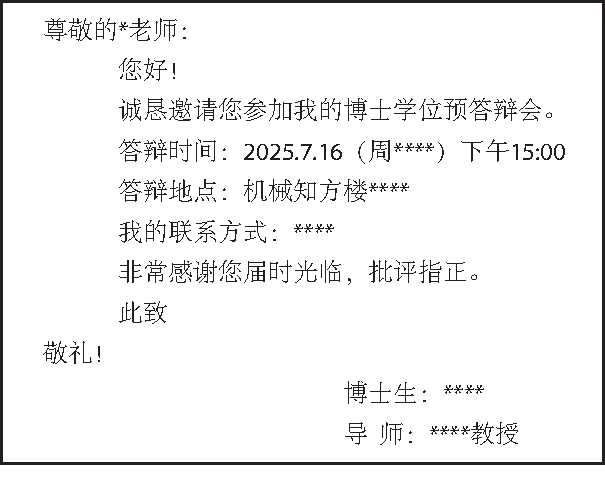
\includegraphics[width=0.5\textwidth]{images/invitationCard}  % 调整Logo宽度
    \caption{答辩邀请卡}
    \label{fig:invitationCard}
  \end{figure}
\item 预约会议室。学生没有权限预约,所以在会议开始前两天的夜间00:00后\footnote{一般只能提前两天}提醒老师预约。同时,可多预约个时间段,自己进行排练。
\item 会议前一天:建议秘书老师再次通知各位老师,以确定时间和地点。如需要借用讲台,可联系于盛军老师。
\item 答辩进行。由秘书负责所有进程。一般为介绍答辩老师,学生基本情况等。然后由主席宣布开始。自己讲解内容40min左右。之后是问答环节,因为是预答,所以老师一般会多提一些问题。不要担心,提多越多,外审的结果越好。开始过程中,秘书会找各位老师填写答辩劳务费表格。
\item 收集老师意见,和检查老师签名等。尽量一次性弄完,不然还要找老师签字。
  \end{enumerate}

    
\section{阶段3:外审}
\label{sec:rev2}

将前面修改好的所有东西修改完毕后,在系统里面提交外审信息。所填写信息比较明朗,上传电子版为主,同时联系韩愈老师通过资格审查等项。

暑假期间一般韩愈老师会通知周几联系她,请注意时间节点。韩愈老师定的时间一般为学校送审时间节点的前两天,不然会延到下周。

已经结业的同学请在门户网站中申请返校答辩,可以提前一同进行,不然时间太紧。

资格通过后,可以上传盲审版。注意要求,可能需要隐去自己导师和自己姓名,全文中的都算,尤其是发表文章处需要格外注意。

送审时间可参见:
\href{https://gs.dlut.edu.cn/info/1207/3992.htm}{博士生学位论文送外审办法及要求}。

提交盲审论文,上传成功后会显示\textbf{盲审论文已上传}(见\autoref{fig:mangshen}),不需要自己再往上提交和确认。

  \begin{figure}[H]
    \centering
    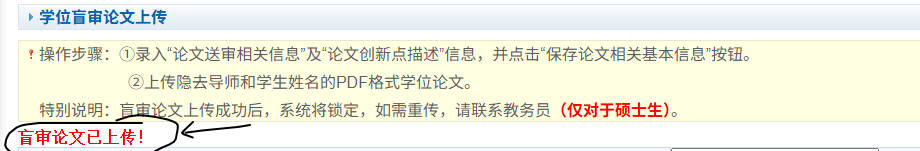
\includegraphics[width=1.0\textwidth]{images/mangshen.jpg}  % 调整Logo宽度
    \caption{盲目上传论文}
    \label{fig:mangshen}
  \end{figure}

 上传之后记住时间节点,一般在7-21天可以返回。没事点击系统里面的【论文盲审评阅书查询】。返回结果一般如:

   \begin{figure}[H]
    \centering
    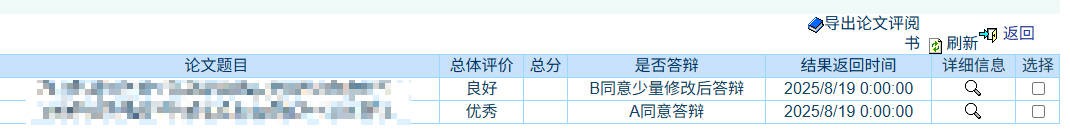
\includegraphics[width=1.0\textwidth]{images/mangshenfanhui.jpg}  % 调整Logo宽度
    \caption{盲审评阅书}
    \label{fig:mangshenfanhui}
  \end{figure}

  按照盲审评阅书的意见返回修改。2A可以5天后答辩、带B的是7天+修改说明、带C的是2月+修改说明、D和E的自己查看相关要求,麻烦的要死,参见大连理工大学学位授予实施细则2025年3月。
\section{阶段4:正式答辩}
\label{sec:realpre}

所需材料有:
\begin{itemize}[label=〇]
\item 评阅书。
\item 答辩情况表。会上交给秘书老师,由秘书老师进行宣读和分发。
\item 纸版论文至少6份。自己1份+各评委老师5份(同样的,加上答辩邀请卡)。
\item 博士学位申请书填写至最后一页。有可能在韩愈老师那边,等待刘巍老师签字。可不需要。
\item 答辩投票表。有的可以使用小程序,纸的可以事先联系秘书或者韩愈老师,多来2份。
\item 答辩PPT。
\item 电子版决议。从答辩情况表中单提出,放到电脑桌面上,以便由会后修改宣读。
\item 录音设备。报退时使用。建议使用两个录音设备,以防意外。
\item HDMI线。连接笔记本和显示屏。
\item 其他物品如茶水、纸巾、水果、纸杯、笔、草稿纸等。
\end{itemize}

大致流程如下:
\begin{enumerate}
\item 仔细阅读学位申请书上最后一页要求,选择导师。如需要有至少两名答辩老师在开题、中期或预答辩中出现;心须有学位分分委员会人员参加\footnote{可向韩愈老师咨询}。
\item 填写学位申请申请书内容。
\item 在确认好导师后,可请自己老师联系和确定时间。自己联系老师和确定时间,不尊重对方老师且浪费时间。
\item 确认好答辩老师后,拟选择会议室\footnote{需要在研究生系统里面填写},在系统中提交答辩信息
\item 向各位老师分发正式论文。推荐在封皮处加上揭示信息,参考实例可见。同时向校外老师咨询是否需要开车进校\footnote{如需要,则索要姓名、车牌、身份证号码、接收短信手机号码}。
\item 预约会议室。学生没有权限预约,所以在会议开始前两天的夜间00:00后\footnote{一般只能提前两天}提醒老师预约。同时,可多预约个时间段,自己进行排练。
\item 在研究生系统填写写答辩公告和答辩申请。同时会导出学位申请书最后一页,可使用此页或修改此页,如部分文字和字体。
  \item 会议前一天:建议秘书老师再次通知各位老师,以确定时间和地点。如需要借用讲台,可联系于盛军老师。
\end{enumerate}

再次提醒:答辩表格内需要导师、评委等签字的地方,尽量评委在场现场签字完成,后续签字很麻烦。。


答辩结束后,根据答辩委员们提出的问题和建议,对学位论文进行认真修改并撰写论文修改说明。



\section{答辩后工件}
\label{sec:realpre}

再次检查达到系统里面包含的信息,是否都填写了。

找韩愈老师领取毕业生登记表、研究生注册卡(这是个啥?哈哈,就是你开学自己手写的那个,死去的记忆慢慢涌来,干!)。仔细填写,不会的先空着,不要瞎定。注意不要涂改;各处需要签名或盖章:本人-班长\footnote{可找李然/于月滨老师咨询。}-辅导员老师\footnote{一般为李然/于月滨老师。}-导师-所在系\footnote{如高性能制造研究所,具体可咨询自己导师。注意,正副所长均可签字。}-学校单位\footnote{大学生活动中心220房间。}-学校(领取时已有)。
\section{阶段5:报退}
\label{sec:resign}

恭喜你。走到这一步,已经变成一个准博士。请放慢一下脚步,给自己的家人、爱人和挚友分享此刻的喜悦吧。

\subsection{导师物品归还}
\label{sec:tutorThings}

比如数据、电脑啥的。也可以没有。但是老师在自己端需要点击确认。

\subsection{图书馆}
\label{sec:library}
书还完。

如有欠费,赶紧给人还上。



\subsection{档案棺材料}
\label{sec:archive}


\textbf{提交之前建议授权书页进行扫描,在图书馆电子论文中等多处需要}。

所有材料不要装订。装订的咋办,你说咋办,扣下来啊。

以下材料需要提交到档案管,并由大学生活动中心学生工件处统一提交。因此,以下材料需要白提交到大学生活动中心-220房间:

\begin{itemize}[label=〇]
\item \textbf{博士学位论文答辩情况表及决议}。各处已经签字。如需签字,下同。
\item \textbf{博士学位论文评阅书}。需要注意的是:1.研究生系统中返回几份,就打印几份;2.如有较大修改或修改后复审,还需要提交签字版修改说明;3.如有不同意答辩,还须提交所有外审意见的评阅书。
\item \textbf{开题、中期评审意见表}。如丢失,可联系同期同学进行补弄。\textbf{若是电子签名,还需要签学院章}。
\item \textbf{博士学位论文胶装版本}。
\item \textbf{答辩光盘}。内有录音、视频\footnote{上交材料时,老师只询问是否有录音和论文。}和电子论文。光盘正面外侧可写上学号-姓名。
\item \textbf{学籍}卡。找韩愈老师领取。
\item \textbf{博士学位申请书}。
  \item \textbf{毕业生登记表}。
  \end{itemize}

  在你提交完存档,学位办老师那边就收到消息,开始打印你的毕业证了。有意思的小彩蛋。
  \subsection{退宿}
\label{sec:tuisu}

退吧。

\subsection{电子论文审核}
\label{sec:Epaper}

电子论文审核,点击图标,会显示办理要求和说明。如果提交之后着急的话,可以向老师打电话。

 \subsection{玉兰卡+网费}
\label{sec:yulan}

之后去大学生活动中心-220房间,注销。

\subsection{进度100\%确认}
\label{sec:jindu100}

确保自己离校系统里面进度是100\%,后面可以领取毕业证和学位证。
  \begin{figure}[H]
    \centering
    
\includegraphics[width=1.0\textwidth]{images/jindu.jpg}  % 调整Logo宽度
    \caption{进度100\%}
    \label{fig:jindu}
  \end{figure}


\subsection{其他乱七八糟}
\label{sec:luanbaqizao}

此项进度不影响领取毕业证和学位证。

其他诸如户口迁移、转档提交等可以同时办理。

同时可以检查研究生系统里面是否能填写的都填写了。

  \section{毕业证-学位证}
\label{sec:certi}

\textbf{毕业证}:研究生大楼-611房间,找苏焱老师领取。老师人很好,嘴甜。


\textbf{学位证}:第一步:上交2份胶装博士论文于韩老师。

第二步:等待老师通知填写一个在线文档,包含个人申请学位论文的信息。此在线文档一般在学位会前一周填写。

第三步:询问韩老师近期的学位会召开时间,一般为3、6、9、12月,且为当月的20-25号。召开学位会当天或次日后,即可联系韩老师领取。次日比较稳妥,韩老师要从研究生办领取回来,然后分发给每位同学。



\section{相关链接}
\label{sec:UsedLinks}
\begin{enumerate}
\item \href{https://ss.dlut.edu.cn/info/1341/24831.htm}{大连理工大学软件学院-博士答辩及报退流程(更新答辩委员要求)-2025.4}
  \item \href{https://gs.dlut.edu.cn/yjspy/pygcguan_li/zytz.htm}{大连理工大学研究生院-重要通知}
\end{enumerate}


\section{相关联系方式}
\label{sec:contact}

学院:韩愈老师0411-84708812

学院:于月滨老师0411-84706820

大学生活动中心:0411-84708167

档案棺:0411-84708906

图书馆电子论文审核:0411-84709862

研究生院学位办:高成锴0411-84708334

\section{致谢}
\label{sec:ack}

仅对文档编写和更正作出贡献的人员致以敬意。

V1.0(2025年09月) \hspace{2cm}编者:王小二的简单生活

V1.1(2025年10月) \hspace{2cm}编者:王小二的简单生活

\end{document}
%%% Local Variables:
%%% mode: LaTeX
%%% TeX-master: t
%%% TeX-master: t
%%% End:
